\documentclass{article}
\usepackage{graphicx} %package to manage images
\graphicspath{ {./figures/} }
\usepackage{hyperref}
\usepackage{caption}
\usepackage[font=scriptsize]{subcaption}
\captionsetup[figure]{labelsep=none}
\captionsetup[table]{labelsep=none}
\usepackage{bbm}
\usepackage{amsmath}
\usepackage{import}
\usepackage{array}
\usepackage{booktabs}
\usepackage{afterpage}
\usepackage{floatrow}
\usepackage{pdflscape}
\usepackage{soul}
\usepackage{float}
\usepackage{adjustbox}
\usepackage{longtable}


\title{maternal nutrition by social group}

\date{June 2025}

\begin{document}

\maketitle


% \section{BMI : 5 covariates, single year age }

% reweighting vars used: age edu rural hasboy c user

% \begin{table}[H]
%     \centering
%     \footnotesize % shrink text
%     \caption{: BMI by group, reweighting vars used: age edu rural hasboy c user}
%     \label{tab:sumstat}
%     \adjustbox{width=\textwidth}{\begin{tabular}{lccc}
\toprule
Group & BMI & \% pregnant sample dropped \\\\
\midrule
Forward: parity 0&22.7 (22.4, 22.9)&.14\\
Forward: parity 1&22.8 (22.6, 23.1)&.09\\
Forward: parity 2&22.6 (22.3, 22.9)&0\\
Forward: parity 3&23.0 (22.3, 23.6)&5.33\\
Forward: parity 4+&22.8 (22.0, 23.5)&4.44\\
OBC: parity 0&21.8 (21.7, 21.9)&.06\\
OBC: parity 1&22.1 (22.0, 22.2)&.04\\
OBC: parity 2&21.9 (21.8, 22.1)&0\\
OBC: parity 3&21.6 (21.4, 21.8)&.91\\
OBC: parity 4+&21.0 (20.4, 21.7)&2.82\\
Dalit: parity 0&21.7 (21.6, 21.9)&0\\
Dalit: parity 1&21.9 (21.8, 22.1)&.25\\
Dalit: parity 2&21.8 (21.6, 21.9)&.14\\
Dalit: parity 3&21.4 (21.1, 21.6)&.36\\
Dalit: parity 4+&21.4 (21.1, 21.7)&2.48\\
Adivasi: parity 0&20.9 (20.7, 21.2)&.26\\
Adivasi: parity 1&22.5 (20.1, 24.9)&.06\\
Adivasi: parity 2&21.1 (20.8, 21.4)&.11\\
Adivasi: parity 3&20.8 (20.3, 21.3)&.5\\
Adivasi: parity 4+&20.7 (20.1, 21.3)&.32\\
Muslim: parity 0&22.3 (22.1, 22.5)&.07\\
Muslim: parity 1&22.8 (22.5, 23.1)&.1\\
Muslim: parity 2&22.9 (22.7, 23.1)&.56\\
Muslim: parity 3&23.0 (22.2, 23.7)&.42\\
Muslim: parity 4+&22.8 (22.0, 23.5)&.85\\
\bottomrule
\end{tabular}
}
% \end{table}


% among forward parity 3, bins that have only pregnant women are of age 26,35,36
% among forward parity 4, bins that have only pregnant women are of age 26,36

% that tells us it's not an age sparsity issue (maybe among 35,36) - let's look to see what other dimension is

% \section{underweight : 5 covariates, single year age }

% reweighting vars used: age edu rural hasboy c user

% \begin{table}[H]
%     \centering
%     \footnotesize % shrink text
%     \caption{: Underweight by group, reweighting vars used: age edu rural hasboy c user}
%     \label{tab:sumstat}
%     \adjustbox{width=\textwidth}{\begin{tabular}{lccc}
\toprule
Group & \% underweight & \% pregnant sample dropped \\\\
\midrule
Forward: parity 0&0.1 (0.1, 0.2)&.14\\
Forward: parity 1&0.1 (0.1, 0.2)&.09\\
Forward: parity 2&0.1 (0.1, 0.2)&0\\
Forward: parity 3&0.1 (0.1, 0.2)&5.33\\
Forward: parity 4+&0.1 (0.0, 0.2)&4.44\\
OBC: parity 0&0.2 (0.2, 0.2)&.06\\
OBC: parity 1&0.2 (0.2, 0.2)&.04\\
OBC: parity 2&0.2 (0.2, 0.2)&0\\
OBC: parity 3&0.2 (0.2, 0.2)&.91\\
OBC: parity 4+&0.2 (0.1, 0.4)&2.82\\
Dalit: parity 0&0.2 (0.2, 0.2)&0\\
Dalit: parity 1&0.2 (0.2, 0.2)&.25\\
Dalit: parity 2&0.2 (0.2, 0.2)&.14\\
Dalit: parity 3&0.2 (0.2, 0.2)&.36\\
Dalit: parity 4+&0.2 (0.2, 0.2)&2.48\\
Adivasi: parity 0&0.2 (0.2, 0.3)&.26\\
Adivasi: parity 1&0.2 (0.1, 0.2)&.06\\
Adivasi: parity 2&0.2 (0.2, 0.3)&.11\\
Adivasi: parity 3&0.3 (0.2, 0.4)&.5\\
Adivasi: parity 4+&0.3 (0.2, 0.4)&.32\\
Muslim: parity 0&0.1 (0.1, 0.1)&.07\\
Muslim: parity 1&0.1 (0.1, 0.1)&.1\\
Muslim: parity 2&0.1 (0.1, 0.1)&.56\\
Muslim: parity 3&0.1 (0.1, 0.1)&.42\\
Muslim: parity 4+&0.1 (0.1, 0.2)&.85\\
\bottomrule
\end{tabular}
}
% \end{table}


% \newpage

% \section{bmi : 5 covariates, 2 year age bins }

% reweighting vars used: age edu rural hasboy c user

% \begin{table}[H]
%     \centering
%     \footnotesize % shrink text
%     \caption{: Underweight by group, reweighting vars used: age edu rural hasboy c user}
%     \label{tab:sumstat}
%     \adjustbox{width=\textwidth}{\input{tables/rw__bmi}}
% \end{table}



% \newpage 
% \section{underweight : 5 covariates, 2 year age bins }

% reweighting vars used: age edu rural hasboy c user

% \begin{table}[H]
%     \centering
%     \footnotesize % shrink text
%     \caption{: Underweight by group, reweighting vars used: age edu rural hasboy c user}
%     \label{tab:sumstat}
%     \adjustbox{width=\textwidth}{\input{tables/rw_}}
% \end{table}


\newpage 
\section{\% underweight : + breastfeeding \& 2 year age bins }

reweighting vars used: age (2yr bins) edu rural hasboy cuser v404 (currently breastfeeding)

\begin{table}[H]
    \centering
    \footnotesize % shrink text
    \caption{: percent underweight by group, reweighting vars used: age edu rural hasboy c user}
    \label{tab:sumstat}
    \adjustbox{width=\textwidth}{\begin{tabular}{lccc}
\toprule
Group &  & \% pregnant sample dropped \\\\
\midrule
Forward: parity 0&15.9 (14.1, 17.7)&.14\\
Forward: parity 1&14.4 (12.9, 15.9)&.09\\
Forward: parity 2&16.1 (13.9, 18.3)&.28\\
Forward: parity 3+&16.2 (12.7, 19.7)&1.86\\
OBC: parity 0&21.4 (20.2, 22.6)&.06\\
OBC: parity 1&19.2 (18.3, 20.1)&.04\\
OBC: parity 2&19.8 (18.5, 21.1)&.1\\
OBC: parity 3+&21.0 (19.1, 22.9)&.32\\
Dalit: parity 0&22.5 (20.9, 24.0)&0\\
Dalit: parity 1&21.2 (19.9, 22.5)&.19\\
Dalit: parity 2&20.5 (18.9, 22.0)&.13\\
Dalit: parity 3+&22.1 (20.4, 23.8)&.72\\
Adivasi: parity 0&29.7 (27.1, 32.2)&.22\\
Adivasi: parity 1&24.9 (22.9, 26.9)&.13\\
Adivasi: parity 2&26.2 (23.8, 28.5)&.11\\
Adivasi: parity 3+&26.2 (24.0, 28.5)&0\\
Muslim: parity 0&15.2 (13.0, 17.3)&.07\\
Muslim: parity 1&14.4 (12.7, 16.1)&.1\\
Muslim: parity 2&13.1 (11.5, 14.6)&.55\\
Muslim: parity 3+&14.4 (12.8, 15.9)&0\\
\bottomrule
\end{tabular}
}
\end{table}

\newpage 
\section{bmi : + breastfeeding \& 2 year age bins }

reweighting vars used: age (2yr bins) edu rural hasboy cuser v404 (currently breastfeeding)

\begin{table}[H]
    \centering
    \footnotesize % shrink text
    \caption{: bmi by group, reweighting vars used: age edu rural hasboy c user}
    \label{tab:sumstat}
    \adjustbox{width=\textwidth}{\begin{tabular}{lccc}
\toprule
Group &  & \% pregnant sample dropped \\\\
\midrule
Forward: parity 0&22.3 (22.1, 22.6)&.14\\
Forward: parity 1&22.8 (22.6, 23.0)&.09\\
Forward: parity 2&22.4 (22.2, 22.7)&.28\\
Forward: parity 3+&22.3 (21.9, 22.7)&1.86\\
OBC: parity 0&21.5 (21.3, 21.6)&.06\\
OBC: parity 1&22.0 (21.9, 22.1)&.04\\
OBC: parity 2&21.8 (21.7, 22.0)&.1\\
OBC: parity 3+&21.4 (21.3, 21.6)&.32\\
Dalit: parity 0&21.5 (21.3, 21.6)&0\\
Dalit: parity 1&21.8 (21.6, 22.0)&.19\\
Dalit: parity 2&21.6 (21.5, 21.8)&.13\\
Dalit: parity 3+&21.3 (21.1, 21.4)&.72\\
Adivasi: parity 0&20.4 (20.2, 20.6)&.22\\
Adivasi: parity 1&20.9 (20.6, 21.1)&.13\\
Adivasi: parity 2&20.8 (20.6, 21.1)&.11\\
Adivasi: parity 3+&20.6 (20.4, 20.8)&0\\
Muslim: parity 0&22.1 (21.8, 22.3)&.07\\
Muslim: parity 1&22.5 (22.2, 22.7)&.1\\
Muslim: parity 2&22.8 (22.6, 23.0)&.55\\
Muslim: parity 3+&22.5 (22.3, 22.7)&0\\
\bottomrule
\end{tabular}
}
\end{table}


\newpage 
\section{weight : + breastfeeding \& 2 year age bins }

reweighting vars used: age (2yr bins) edu rural hasboy cuser v404 (currently breastfeeding)

\begin{table}[H]
    \centering
    \footnotesize % shrink text
    \caption{: bmi by group, reweighting vars used: age edu rural hasboy c user}
    \label{tab:sumstat}
    \adjustbox{width=\textwidth}{\begin{tabular}{lccc}
\toprule
Group & \% underweight & \% pregnant sample dropped \\\\
\midrule
Forward: parity 0&52.8 (52.3, 53.3)&0\\
Forward: parity 1&53.8 (53.1, 54.5)&.27\\
Forward: parity 2&53.0 (52.1, 53.9)&.62\\
Forward: parity 3+&53.3 (51.5, 55.1)&3.33\\
OBC: parity 0&50.8 (50.5, 51.1)&0\\
OBC: parity 1&50.5 (48.3, 52.7)&.08\\
OBC: parity 2&50.9 (50.5, 51.3)&0\\
OBC: parity 3+&49.8 (49.2, 50.4)&.99\\
Dalit: parity 0&49.7 (49.4, 50.0)&0\\
Dalit: parity 1&50.9 (50.4, 51.3)&.25\\
Dalit: parity 2&49.9 (49.4, 50.4)&.55\\
Dalit: parity 3+&48.7 (48.3, 49.2)&.91\\
Adivasi: parity 0&47.7 (47.1, 48.2)&.1\\
Adivasi: parity 1&50.2 (47.2, 53.1)&.13\\
Adivasi: parity 2&48.9 (48.1, 49.7)&.77\\
Adivasi: parity 3+&48.7 (47.8, 49.6)&.69\\
Muslim: parity 0&51.6 (51.2, 52.1)&0\\
Muslim: parity 1&53.1 (52.5, 53.7)&.19\\
Muslim: parity 2&53.9 (53.3, 54.5)&.69\\
Muslim: parity 3+&52.6 (51.9, 53.2)&.84\\
\bottomrule
\end{tabular}
}
\end{table}



\section{outcome: BMI}
\begin{figure}[H]
    \centering
    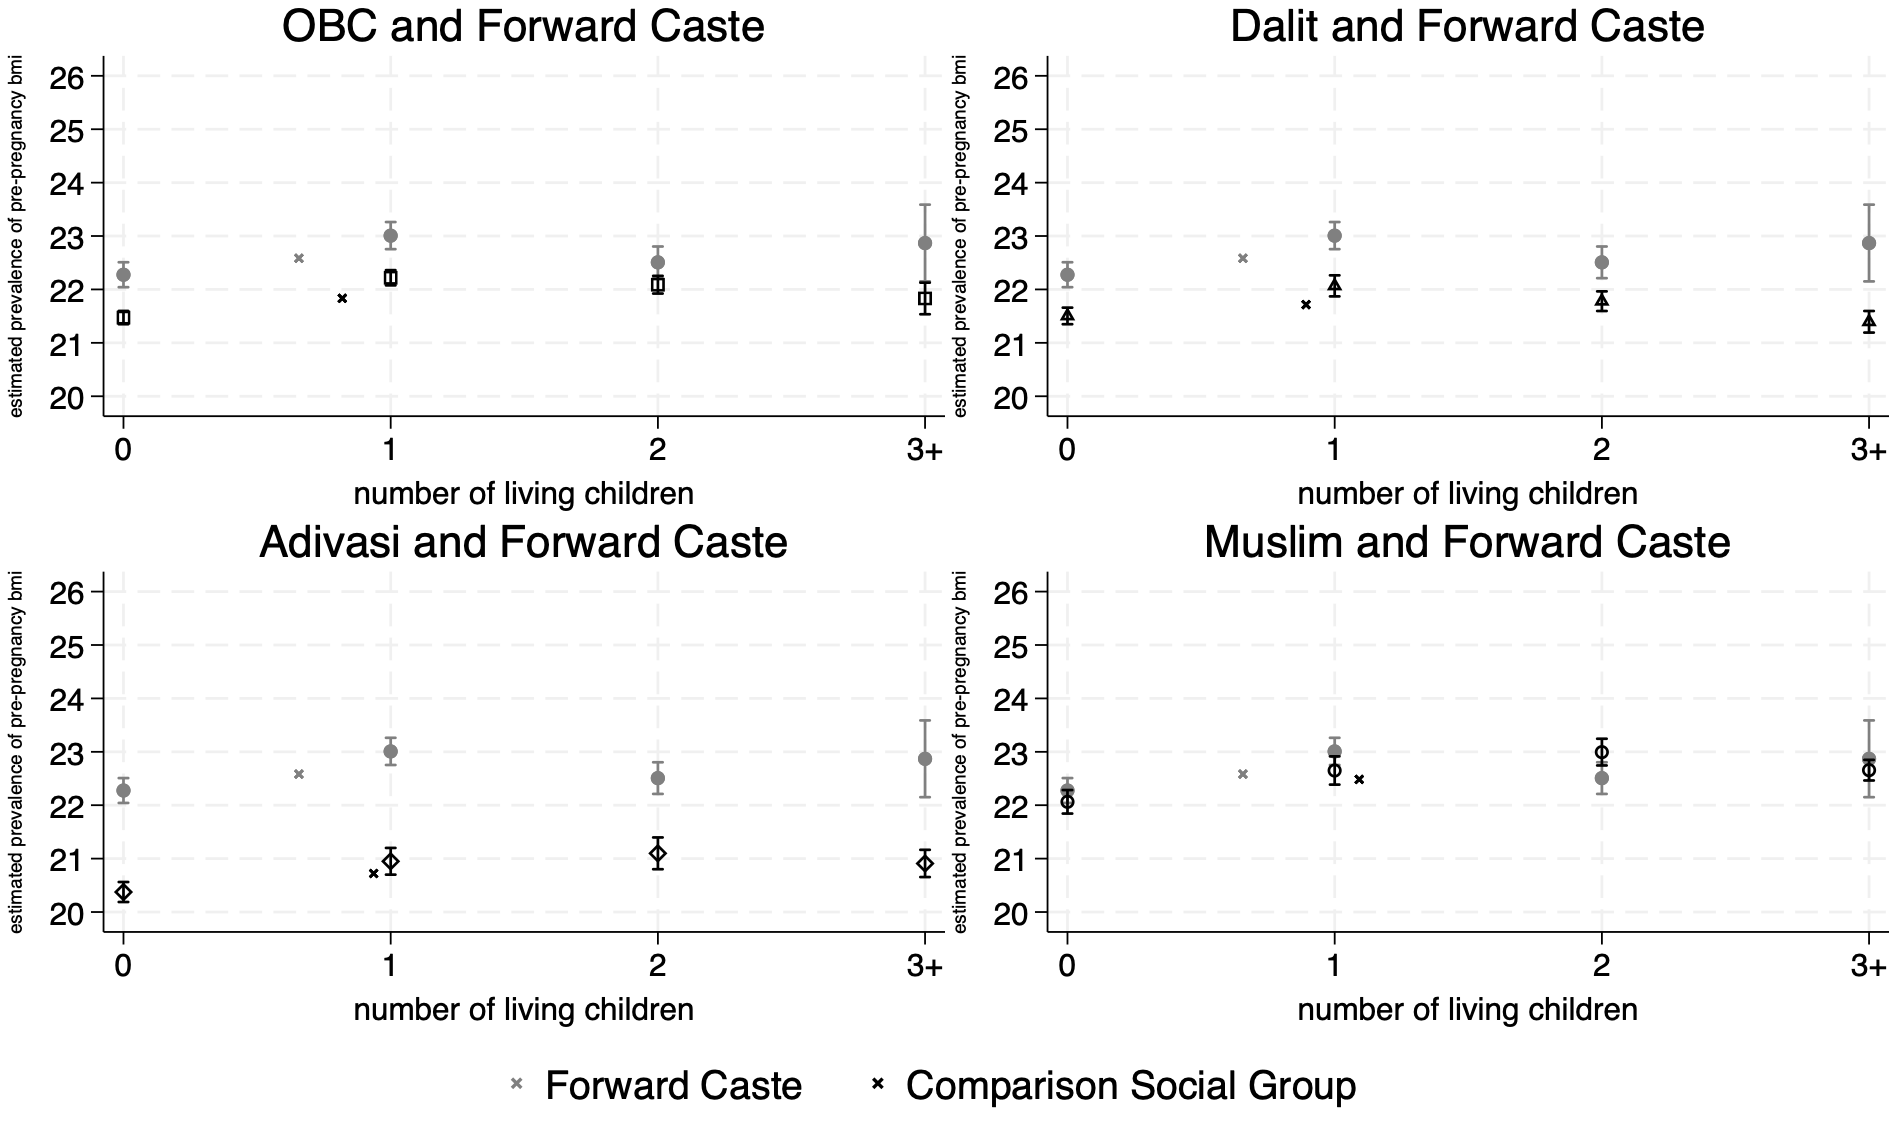
\includegraphics[width=\textwidth]{figures/prepreg_bmi_combined.png}
\end{figure}

\section{outcome: underweight}
\begin{figure}[H]
    \centering
    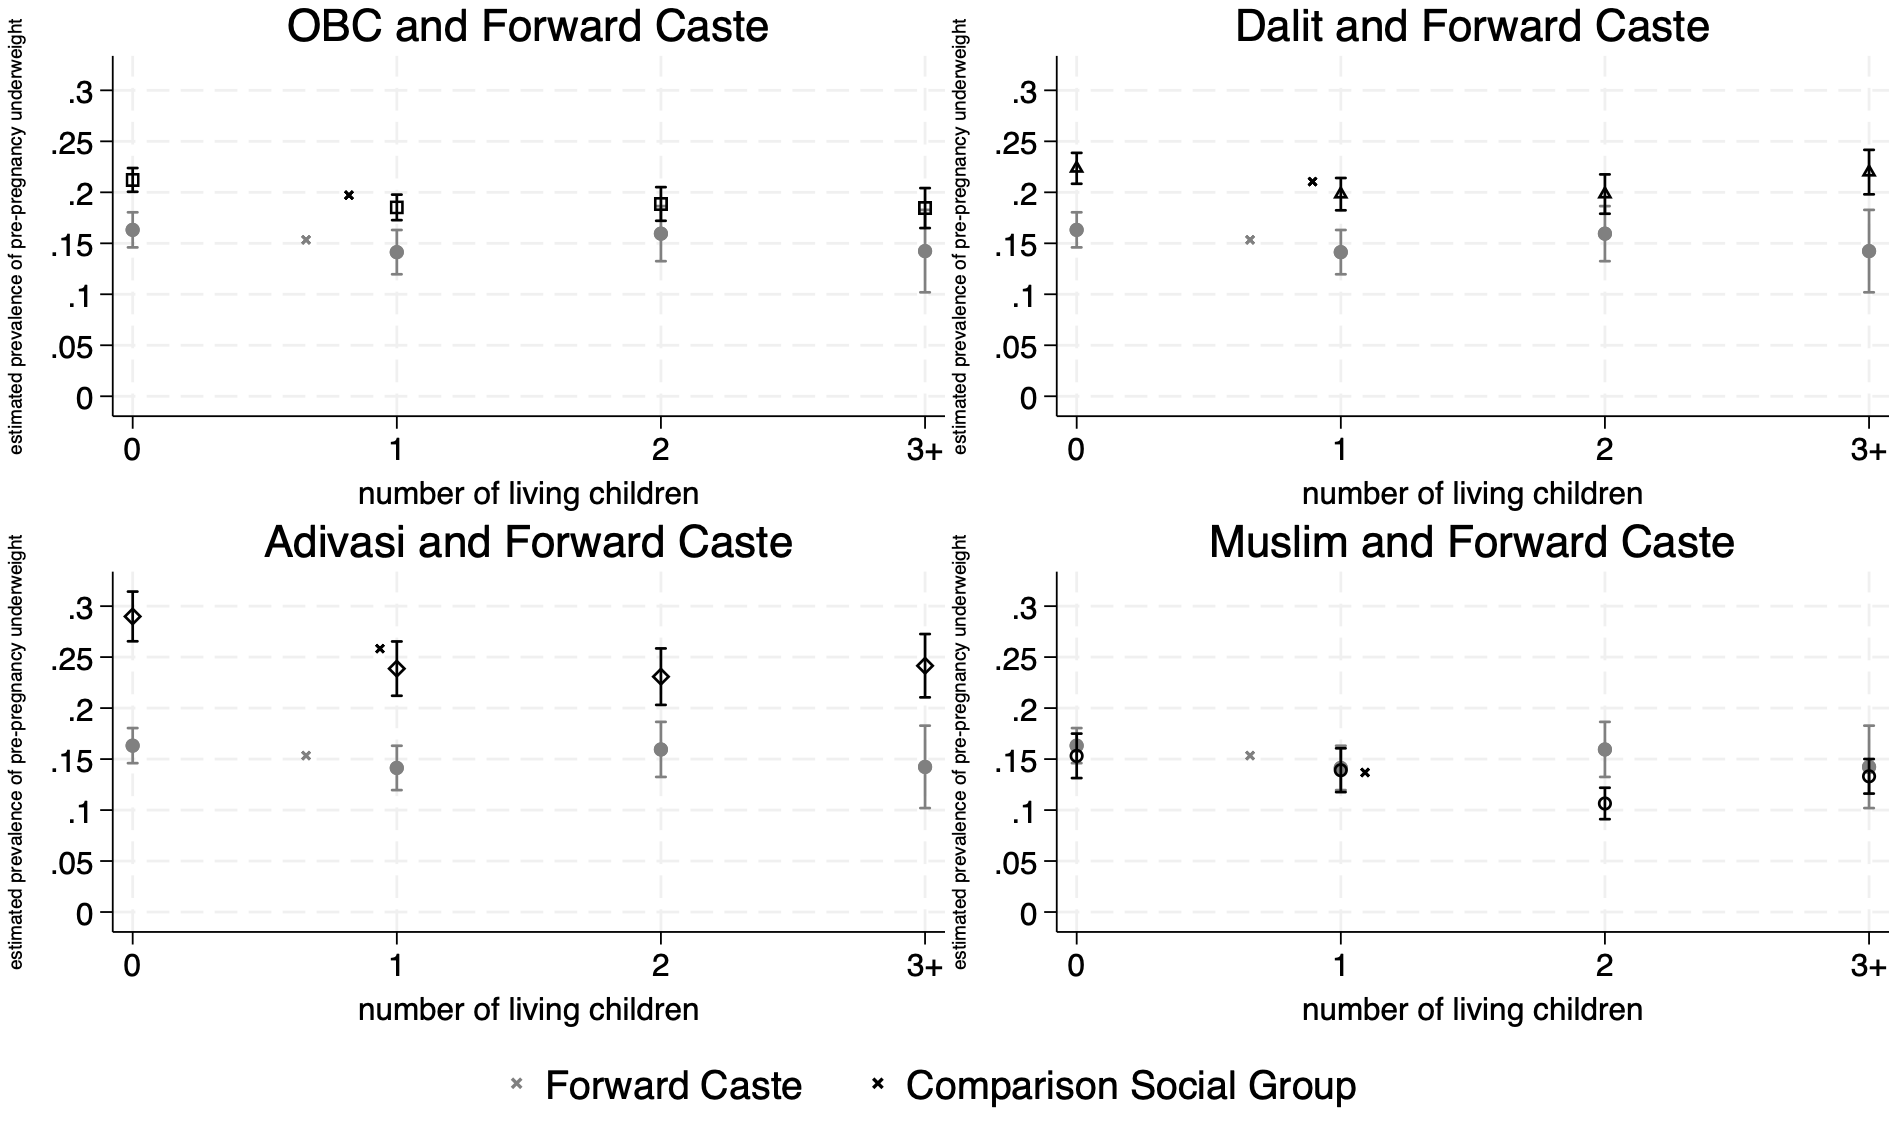
\includegraphics[width=\textwidth]{figures/:prepreg_underweight_combined.png}
\end{figure}

\section{stacked bar graph}
\begin{figure}[H]
    \centering
    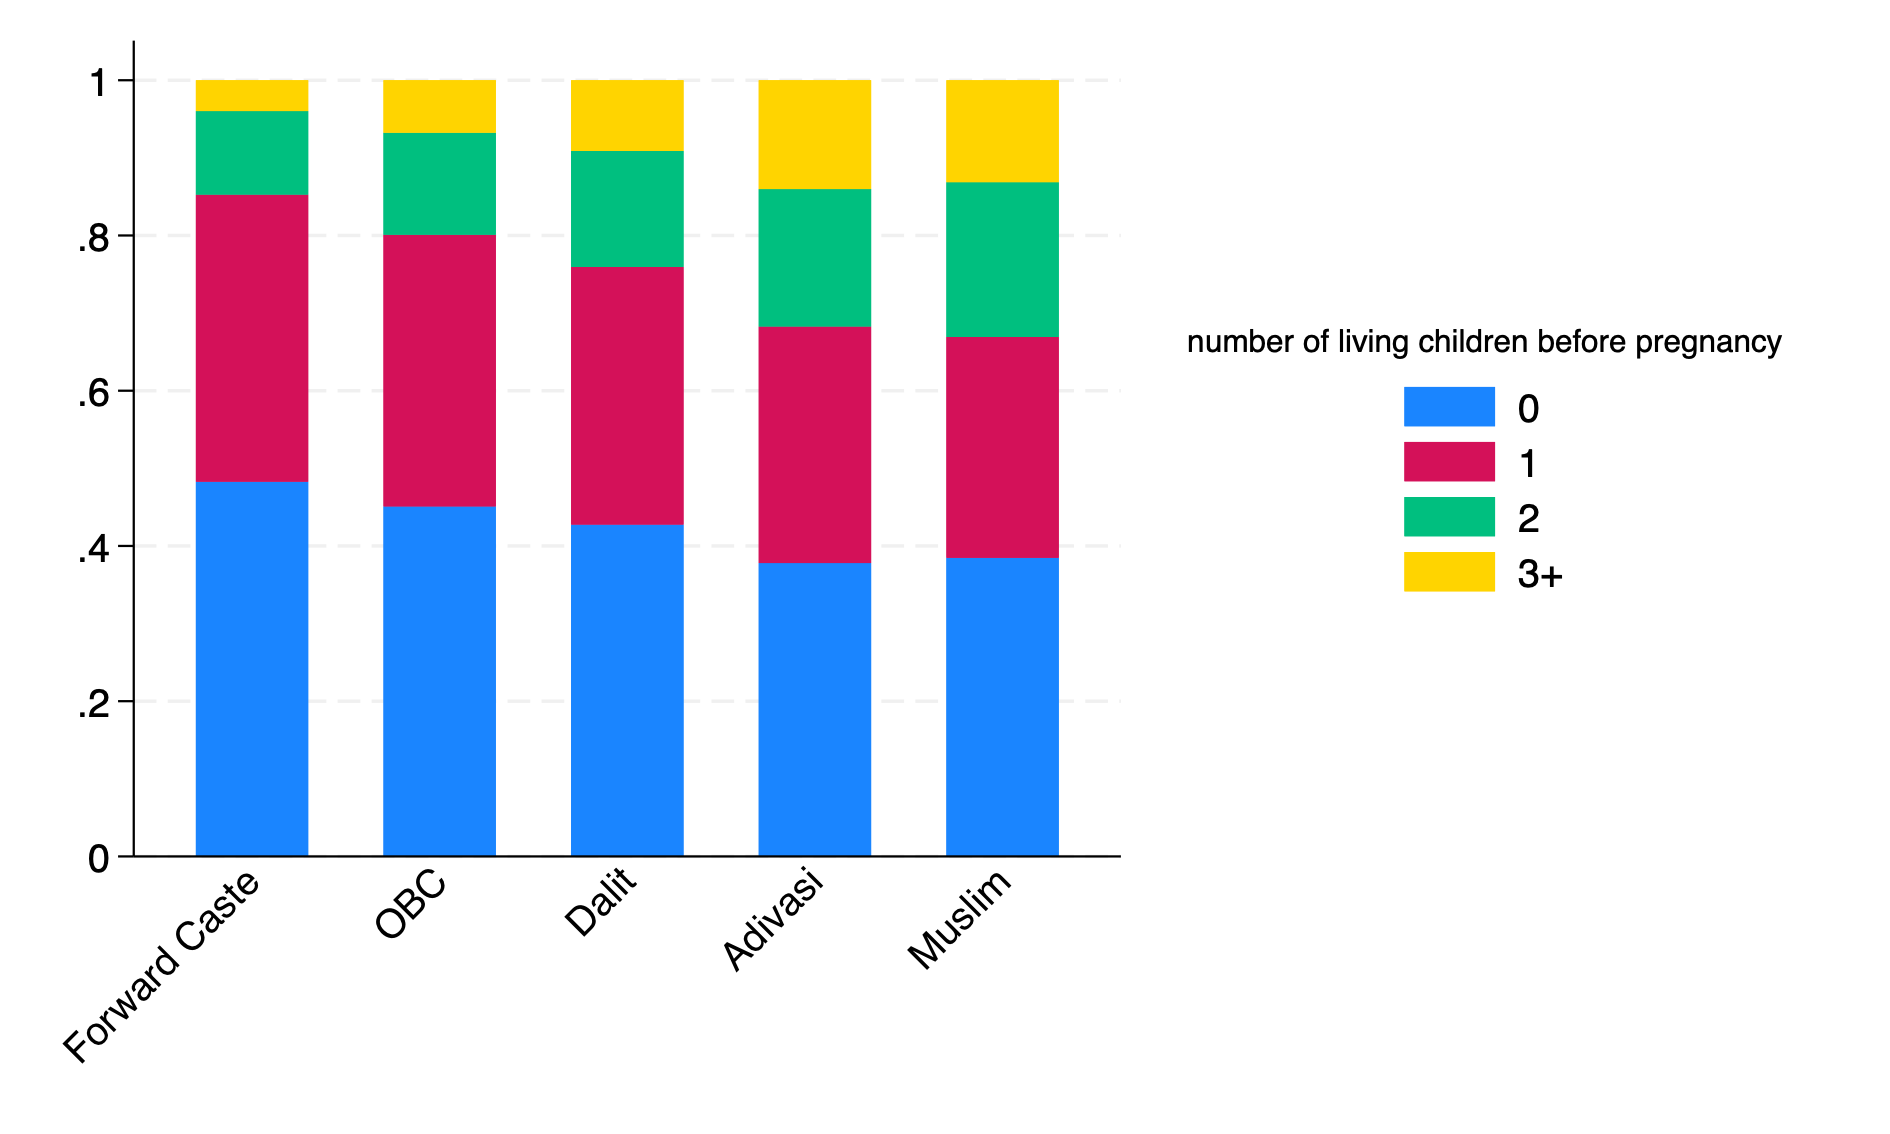
\includegraphics[width=\textwidth]{figures/stackedbar_parity_socialgroup.png}
\end{figure}


\newpage
\section{kitagawa}



\begin{table}[H]
    \centering
    \footnotesize % shrink text
    \caption{: Dalit fwd decomposition}
    \label{tab:sumstat}
    \adjustbox{width=\textwidth}{\begin{tabular}{l*{6}{c}}
\toprule
            &\multicolumn{1}{c}{Parity 0}&\multicolumn{1}{c}{Parity 1}&\multicolumn{1}{c}{Parity 2}&\multicolumn{1}{c}{Parity 3+}&\multicolumn{1}{c}{total}&\multicolumn{1}{c}{pct}\\
\midrule
\midrule
Fwd prop. pregnant women&        0.50&        0.37&        0.09&        0.04&            &            \\
Fwd avg pre-pregnancy bmi&       22.28&       23.01&       22.51&       22.87&       22.59&            \\
Dalit prop. pregnant women&        0.43&        0.34&        0.15&        0.09&            &            \\
Dalit avg pre-pregnancy bmi&       21.50&       22.07&       21.78&       21.39&       21.72&            \\
total\_diff  &       -0.77&       -0.94&       -0.73&       -1.47&        0.87&            \\
within\_group&       -0.36&       -0.33&       -0.08&       -0.09&       -0.87&     -100.44\\
between\_group&       -1.63&       -0.82&        1.36&        1.09&        0.00&        0.44\\
\bottomrule
\end{tabular}
}
\end{table}

\begin{table}[H]
    \centering
    \footnotesize % shrink text
    \caption{: Adivasi fwd decomposition}
    \label{tab:sumstat}
    \adjustbox{width=\textwidth}{\begin{tabular}{l*{6}{c}}
\toprule
            &\multicolumn{1}{c}{Parity 0}&\multicolumn{1}{c}{Parity 1}&\multicolumn{1}{c}{Parity 2}&\multicolumn{1}{c}{Parity 3+}&\multicolumn{1}{c}{total}&\multicolumn{1}{c}{pct}\\
\midrule
\midrule
Fwd prop. pregnant women&        0.50&        0.37&        0.09&        0.04&            &            \\
Fwd avg pre-pregnancy underweight&        0.16&        0.14&        0.16&        0.14&        0.15&            \\
Adivasi prop. pregnant women&        0.41&        0.34&        0.15&        0.10&            &            \\
Adivasi avg pre-pregnancy underweight&        0.29&        0.24&        0.23&        0.24&        0.26&            \\
total\_diff  &        0.13&        0.10&        0.07&        0.10&       -0.10&            \\
within\_group&        0.06&        0.03&        0.01&        0.01&        0.11&     -102.83\\
between\_group&       -0.02&       -0.01&        0.01&        0.01&       -0.00&        2.83\\
\bottomrule
\end{tabular}
}
\end{table}



\begin{table}[H]
    \centering
    \footnotesize % shrink text
    \caption{: Muslim fwd decomposition}
    \label{tab:sumstat}
    \adjustbox{width=\textwidth}{\begin{tabular}{l*{6}{c}}
\toprule
            &\multicolumn{1}{c}{Parity 0}&\multicolumn{1}{c}{Parity 1}&\multicolumn{1}{c}{Parity 2}&\multicolumn{1}{c}{Parity 3+}&\multicolumn{1}{c}{total}&\multicolumn{1}{c}{pct}\\
\midrule
\midrule
Fwd prop. pregnant women&        0.50&        0.37&        0.09&        0.04&            &            \\
Fwd avg pre-pregnancy bmi&       22.28&       23.01&       22.51&       22.87&       22.59&            \\
Muslim prop. pregnant women&        0.39&        0.28&        0.19&        0.14&            &            \\
Muslim avg pre-pregnancy bmi&       22.06&       22.65&       22.99&       22.66&       22.49&            \\
total\_diff  &       -0.21&       -0.36&        0.49&       -0.21&        0.10&            \\
within\_group&       -0.09&       -0.12&        0.07&       -0.02&       -0.16&     -161.98\\
between\_group&       -2.59&       -2.19&        2.48&        2.36&        0.06&       61.98\\
\bottomrule
\end{tabular}
}
\end{table}

\begin{table}[H]
    \centering
    \footnotesize % shrink text
    \caption{: OBC fwd decomposition}
    \label{tab:sumstat}
    \adjustbox{width=\textwidth}{\begin{tabular}{l*{6}{c}}
\toprule
            &\multicolumn{1}{c}{Parity 0}&\multicolumn{1}{c}{Parity 1}&\multicolumn{1}{c}{Parity 2}&\multicolumn{1}{c}{Parity 3+}&\multicolumn{1}{c}{total}&\multicolumn{1}{c}{pct}\\
\midrule
\midrule
Fwd prop. pregnant women&        0.50&        0.37&        0.09&        0.04&            &            \\
Fwd avg pre-pregnancy underweight&        0.16&        0.14&        0.16&        0.14&        0.15&            \\
OBC prop. pregnant women&        0.45&        0.35&        0.13&        0.07&            &            \\
OBC avg pre-pregnancy underweight&        0.21&        0.19&        0.19&        0.18&        0.20&            \\
total\_diff  &        0.05&        0.04&        0.03&        0.04&       -0.04&            \\
within\_group&        0.02&        0.02&        0.00&        0.00&        0.04&     -101.91\\
between\_group&       -0.01&       -0.00&        0.01&        0.00&       -0.00&        1.91\\
\bottomrule
\end{tabular}
}
\end{table}





\end{document}
